\chapter{Theoretical background}
\label{chap:dataanalysis}

Data analysis is becoming increasingly popular due to the rapid growth of data amounts and the natural need for extracting meaningful information and knowledge from this data. 
Various applications ranging from production control to intrusion detection systems and pattern recognition may benefit from the extracted information and learned knowledge. 
Data analysis may be seen as a step forward in the evolution of information technology. In this chapter some of the most important problems in pattern recognition are presented, namely, clustering and classification. The field of soft computing is  briefly presented in Section \ref{chap:softcomputing} and the topic of multi agent interactions is presented in Section \ref{chap:multiagentinteractions}.

\section{Data analysis and data mining}

The process of gathering, modelling and transforming data in the attempt to extract relevant information that may support decision making is called data analysis. Data mining focuses on modelling predictive rather than purely descriptive purposes and it is a particular technique of data analysis. 
Business intelligence refers to data analysis techniques applied mainly in analysing business data aiming to increase decision making support. Data analysis may be divided into exploratory data analysis and confirmatory data analysis. Exploratory data analysis deals with discovering new features in the data. On the other hand, confirmatory data analysis  deals with confirming or falsifying given hypotheses. However there are several data analysis varieties. Predictive analytics, for example, applies statistical models in forecasting future events. Text analytics focuses on applying various techniques to extract and classify information contained in sources of textual data.

Data being analysed could come from various sources like databases, information repositories, data streams etc. Data warehouses represent an emerging architecture which includes the following processes: data cleaning, integration, and online analytical processing. 
Online analytical processing techniques allow users to analyse information from different perspectives involving the following operations: consolidation, drill-down, slice and dice. Classical classification and clustering methods may further help in data processing and information extraction. 
However, data sources to be analysed go beyond databases or data warehouses. Huge volumes of data may come from data streams or even from the world wide web. Efficient data analysis methods are extremely important in these situations. The huge amounts of data together with the need of extracting meaningful information from the data, is commonly known as ``the data rich  but information poor problem'' \cite{Han06DataMining}. In order to be able to cope with the increasing volumes of data coming from various sources, data analysis methods to be sought need to be scalable, efficient and robust. Data analysis lies at the confluence of several disciplines like databases, statistics, pattern recognition, neural networks, machine learning, image processing, information retrieval and signal processing. So, data analysis is a highly interdisciplinary domain and a natural step forward in the evolution of computer science. 

Intelligent data analysis (IDA) is an emerging discipline applied in many fields \cite{website:clustering,Han06DataMining, Gaceanu11Using} ranging from  marketing, finance, stock exchange, insurance to www document classification, biology and so on. 
Traditional data analysis is becoming less able to deal with the challenges raised by the increasing volumes of data and intelligent methods need to be employed in order to handle consequent difficulties. Thus intelligent data analysis deals with the development of intelligent systems for data analysis. The concepts of interest in this area include: classical statistical models, neural networks, fuzzy systems, evolutionary computation, cluster analysis, intelligent agents, expert systems, and rough sets.


\section{Pattern recognition}
Pattern recognition is the problem of assigning a label to a given input data. 	
According to the type of the involved learning procedure, algorithms in pattern recognition may be categorized in supervised learning, unsupervised learning and semi-supervised learning algorithms. In the following we will refer to clustering which is an unsupervised learning problem and to classifications which is a supervised learning problem.

\subsection{Cluster analysis}

According to \cite{website:clustering}, clustering is ``the most important unsupervised learning problem''. Given a collection of unlabelled data the goal of a clustering process is to find a structure in the considered dataset. In \cite{website:clustering} clustering is defined as ``the process of organizing objects into groups whose members are similar in some way''. So a cluster is a group of objects which are ``similar'' between them and are ``dissimilar'' to the objects belonging to other clusters \cite{website:clustering}.

A good clustering algorithm should satisfy several requirements as follows \cite{website:clustering}:

\begin{itemize}
\item scalability, i.e., it should still work properly when applied to large datasets
\item ability to handle different types of features, namely, continuous, binary, categorical, ordinal and ratio-scaled
\item tolerance to high dimensional data
\item independence with respect to the cluster shape
\item minimal domain knowledge requirements, i.e., not too many parameters that need to be initialized
\item tolerance to noise 
\item tolerance to outliers
\item insensitivity to the order in which data items are read
\item interoperability 
\item usability.
\end{itemize}

There are many fields  in which clustering algorithms may be applied \cite{website:clustering,Han06DataMining}:
\begin{itemize}
\item marketing: given a dataset containing information about customers and their shopping history, find groups of customers that have a similar behaviour
\item biology: given a dataset containing information about plants or animals, classify plants or animals into groups sharing similar features
\item insurance: given a dataset containing information about policy holders, identify groups of persons having high claim costs, i.e., fraud detection
\item earthquake studies: given a dataset of observed earthquake epicenters, the goal is to identify dangerous zones
\item world wide web: identify similar documents or websites; given weblog data, identify groups where access patterns are alike.
\end{itemize}

Clustering can also be used for outlier detection \cite{Zoubi}. A strange data value that stands out, an extreme value, a point which is far away from the other data points or, in general, a data item which is not like the rest of the data items in some sense is commonly known as an outlier \cite{Aggarwal01Outlier}. An outlier may appear as an extreme value or a peculiar combination of the values in multivariate data. 
An important intelligent data analysis task is the handling of such anomalous data items because of the significant influence of outliers on the analysis result.

Careful outlier analysis may lead to the discovery of interesting phenomena from the application domain point of view. Nevertheless it is often the case that outliers are no more than measurement errors.
So simply rejecting all outliers may case important information loss and inaccurate data analysis results. For example, in fraud detection, suspicious credit card transactions may indeed be fraudulent, but could also only be looking suspicious, but actually be legitimate ones. 

Originated as a branch of statistics, clustering tools based on algorithms like k-means or k-medoids have been built into several packages for statistical analysis software like S-Plus, SPSS, SAS etc \cite{Han01Spatial}. Being an unsupervised learning problem, clustering  does neither rely on any predefined classes nor on training examples. So in clustering, learning is observation-based rather than example-based. 
Continuous efforts are being done in order to develop more efficient, robust and scalable clustering analysis techniques.

Clustering methods could be classified in partitioning methods, hierarchical methods, density-based methods, grid-based methods and model-based methods. In the following each class of clustering algorithms will briefly described.

A partitioning clustering algorithm constructs $k$ clusters from the given dataset, where $k <= n$ and $n$ is the number of data items, i.e., objects to be clustered. Given the number of clusters, $k$, a partitioning clustering algorithm starts by creating $k$ initial clusters. Afterwards, it tries to improve the partitioning quality by moving objects from one cluster to another such that objects which are closely related are in the same cluster and objects which are different from each other are located in different clusters.

There are many variations, but two of the most popular would be:
\begin{itemize}
\item k-means
\item k-medoids.
\end{itemize}

In k-means, the representative of a cluster $c$ is the mean value of the data items from $c$.  In the k-medoids clustering algorithm the cluster representative is one of the data items located close to the cluster center.

Both k-means and k-medoids work by minimizing the squared error:
\[
\argmin_C \sum_{i=1}^{k} \sum_{x_j \in C_i} || x_j - \mu_i ||^{2}
\]
where $(x_1, x_2, ..., x_n)$ are the data items to be clustered, $C = \{C_1, C_2, ..., C_k\}$ denotes the set of $k$ clusters ($k \leq n$) and $\mu_i$ is the mean of points in $C_i$.

Partitioning clustering methods are a good choice when the number of clusters in known in advance and when the cluster shape is spherical. However, when the dataset size grows and when the data items are complex, other partitioning methods are needed.

Hierarchical clustering methods create a hierarchy of clusters by repetitive merges or splits, and the whole process may be visualized in a dendrogram. Based on the way the clusters are created (by merging or splitting) hierarchical clustering is either agglomerative or divisive. In the divisive (top-down) approach the algorithm starts from one cluster containing the whole dataset and at each step the clusters are split into smaller ones based on some criterion. The process ends when a certain condition is met or when there is only one data item left in each cluster. In the agglomerative (bottom-up) approach the algorithm starts by encapsulating each data item with a cluster and at each step clusters are merged based on some criterion. The whole process ends when some condition is met or when there is only one cluster left containing the whole dataset.

A major drawback of hierarchical methods is that there is no possibility for undoing either a merge or a split operation so when an erroneous decision has been made there is no way for correction. On the other hand, this situation may also lead to lower computational costs.

The hierarchical clustering quality may be improved in  the following ways:
\begin{itemize}
\item analyse object ``linkages'' at each hierarchical partitioning, like in Chameleon \cite{Karypis99Chameleon}. Chameleon uses a sparse graph in which the nodes represent the data items to be clustered and the edges have associated weights which represent the similarities between the data items. Its key feature is that it takes into account not only interconnectivity but also closeness when deciding if two clusters are similar or not.
\item perform a micro-clustering using an agglomerative approach and then group micro-clusters into macro-clusters  using another clustering method as in BIRCH \cite{Zhang97BIRCH}. 
\end{itemize}

Density-based methods construct clusters by adding data items as long as the number of items in the neighbourhood (the density) exceeds a previously established threshold. In other words, a cluster is valid if given a data item from a cluster the neighbourhood of a certain radius contains at least a certain minimum number of data items. Such a method may be used to filter out outliers and discover clusters having any shape. DBSCAN \cite{Ester09Density} is a density-based clustering algorithm which works well if the density within the clusters is uniform. OPTICS \cite{Ankerst99OPTICS} is another density-based algorithm which addresses the varying density issue from DBSCAN by creating an ordering of the database representing its density density-based clusters.

Grid-based methods perform a grid representation of the object space. This class of methods is especially appropriate when dealing with large data sets. Clustering operations are performed on the grid structure and among the advantages of this method is the fast processing time, which is  dependent on the number of cells in each dimension from the grid space rather than on the number of objects. STING \cite{Wang97STING} is an example of a grid-based method. 

Model-based clustering algorithms consider a model for each cluster and the task of the algorithm is to find the best fit of the given  data with respect to the considered model \cite{Han01Spatial}. The number of clusters is estimated using statistical methods. For example, based on statistical modelling, the EM (expectation-maximization) algorithm performs either expectation or maximization operations at each step. The COBWEB algorithm uses probabilistic concepts as cluster models and incrementally organizes the data items into a classification tree. Self-organizing feature map (SOM) is a neural network-based algorithm that perform a mapping of the data  from high dimensions into a two or three dimension feature map. 


\subsection{Classification}

Classification is the process of assigning a piece of input data (instance or data item) described by a vector of features to a given category (class). Initially a classifier is built based on a given dataset. This step is the training (learning) phase and at this point a classifier is built by learning from a training dataset containing a set of data items with their features and the associated class labels.
Because the class label of each training data item is provided, classification is a supervised learning problem. 
More formally, classification may be seen as learning a mapping, $y = f(X)$, such that given a data item from $X$ the class label $y$ can be predicted. This model is then used for classification. 

The performance or the quality of a classifier can be evaluated by computing its accuracy, i.e., the percentage of test set data items that are correctly classified. Other performance measures could be the computation speed, robustness (the ability to handle noisy or missing data), scalability and interpretability (the level of understanding and insight that is provided by the classifier) \cite{Han06DataMining}.

\subsubsection{Decision tree induction}

Decisions trees are perhaps the most straightforward and intuitive way of representing a classification process and for this reason they have been chosen for introducing this topic.
Decision tree induction is the process of learning decision trees from training datasets. In a decision tree each non-leaf node represents a test on a feature,  branches denote the outcome of a certain  test,  and leaf nodes contain the class labels. An example of a decision tree may be seen in Figure ~\ref{fig:decisiontree} taken from \cite{Han06DataMining}. The concept of ``buys computer'' is represented in this decision tree, i.e., decide whether a given customer is likely to buy a computer. 

%\begin{figure}[h!]
%  \centering
%  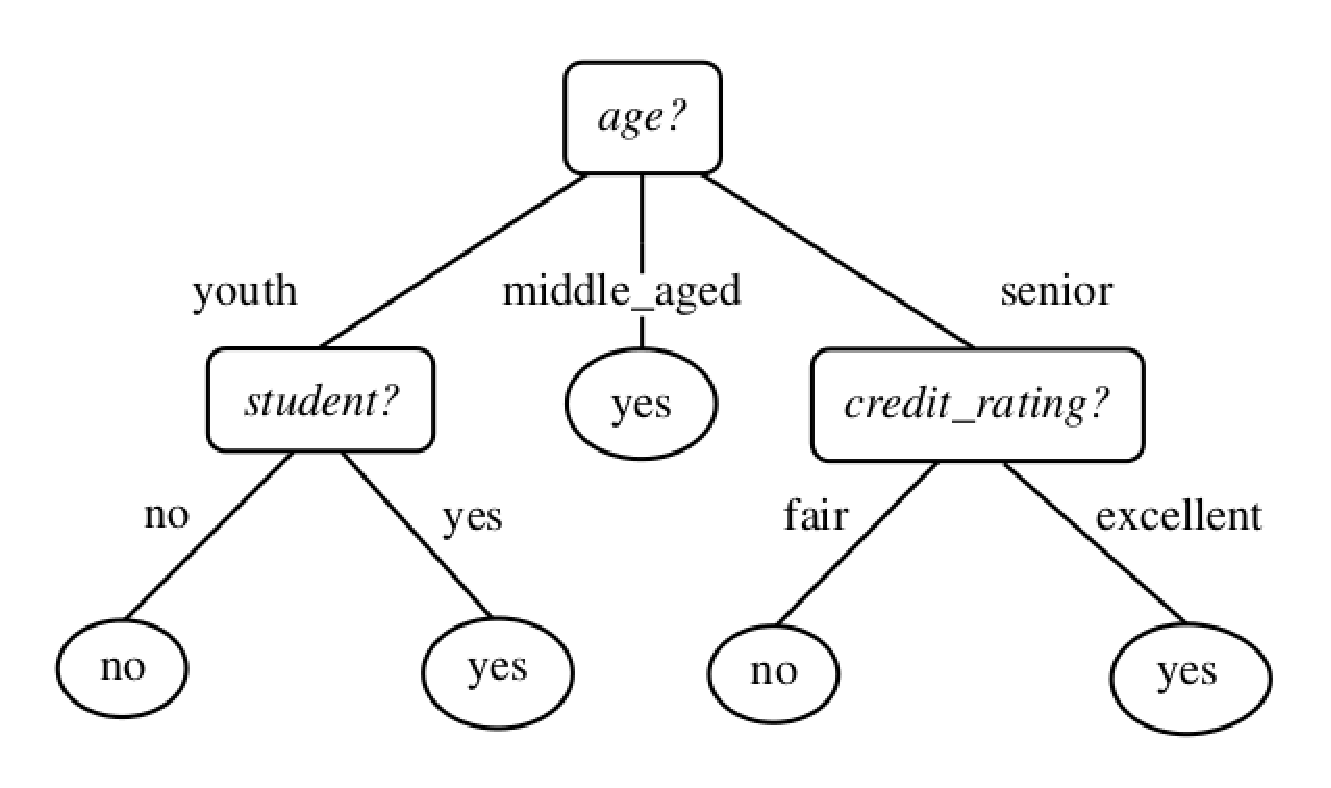
\includegraphics[width=0.5\textwidth]{decisiontree}
%  \caption[Decision tree]{A decision tree for the concept $buys\_computer$, indicating whether a customer is likely to %purchase a computer. Each internal (non-leaf) node represents a test on an feature. Each leaf node represents a class %(either $buys\_computer = yes$ or $buys\_computer = no$).}
%  \label{fig:decisiontree}
%\end{figure}
\begin{figure}[h!]
\centerline{\psfig{figure=decisiontree.eps,width=0.5\textwidth}}
      \caption[Decision tree]{A decision tree for the concept $buys\_computer$, indicating whether a customer is likely to purchase a computer. Each internal (non-leaf) node represents a test on an feature. Each leaf node represents a class (either $buys\_computer = yes$ or $buys\_computer = no$). Image source: \cite{Han06DataMining}.}
\label{fig:decisiontree}
\end{figure}


The classification process takes place in the following way: given a data item with no associated class label, test the data item's features with respect to an already built decision tree. By doing so a path from the root node of the decision tree to a leaf is constructed. The class prediction of the given data item is contained in the leaf node that was reached. It is important to remark that decision trees may be transformed into classification rules. One of the advantages of decision tree classifiers is that they do not require any parameter setting or domain knowledge, making them suitable for exploratory knowledge discovery \cite{Han06DataMining}. Another advantage is their ability to handle high dimensional data. Also the tree representation is intuitive and easily understandable. According to \cite{Han06DataMining} decision tree classifiers have good accuracy. During tree construction, various feature selection methods are used in order to select the feature that leads to the best data partitioning. When building decision trees, some branches may represent noise or may denote outliers from the training dataset and hence tree pruning is used for removing these branches. A drawback of decision trees is scalability since in general the dataset is memory resident. A general approach for decision trees construction is presented in Algorithm ~\ref{alg:decisiontree}.

\begin{algorithm}
\caption{Generate decision tree}
\label{alg:decisiontree}
\begin{algorithmic}[1]
\STATE Create a node $N$
\STATE Check for particular cases
\STATE Find the feature $a_{best}$ that best divides the training data
\STATE Label the node $N$ with $a_{best}$
\STATE Recurse on the split data and add the new nodes as children of node $N$
\end{algorithmic}
\end{algorithm}

A particular case is when all data items from the dataset are of the same class $C$. In this case the node $N$ is returned with label $C$. Another particular case is when the feature list is empty and in this particular case the node $N$ is labelled by the majority class, $C$, from the dataset.

An important step of the considered algorithm is choosing the splitting feature $a_{best}$ that best divides the input data.
Decision tree algorithms differ from each other mainly in two aspects: the feature selection process and pruning mechanism.
In a feature selection process the goal is to select the splitting criterion that best partitions a given dataset, $D$, of class-labelled training data items into separate partitions. 
In the ideal case the resulted partitions are pure, i.e., all data items from a partition belong to the same class.
Some of the mostly used feature selection measures (splitting rules) are information gain, gain ratio, and gini index \cite{Han06DataMining}.

Let $D$ be a training dataset of class-labelled data items and $m$ the number of classes, $C_{i}, i = \overline{1,m} $. 

The $ID3$ algorithm uses information gain as its feature selection measure by determining at each step the attribute having the highest information gain and grouping data items according to the value of the selected attribute \cite{Han06DataMining}. 

\begin{definition}
The expected information needed for classifying a data item in $D$ (the entropy of $D$) is given by
\begin{align}
Info(D) = - \sum_{i=1}^{m}p_{i}\log_{2}(p_{i}),
\end{align}
where: 
\begin{itemize}
\item $p_{i}$ denotes the probability that a data item from the dataset belongs to the class $C_{i}$
\item $p_{i} \approx \frac{\mid C_{i} \mid }{\mid D \mid} $.
\end{itemize}
\end{definition}

\begin{definition}
The expected information needed for partitioning a dataset $D$ given an attribute $A$ is
\begin{align}
Info_{A}(D)=\sum_{j=1}^{v} \frac{\mid D_{j} \mid}{\mid D \mid} Info(D_{j}),
\end{align}
where:
\begin{itemize}
\item the term $\frac{\mid D_{j} \mid}{\mid D \mid}$ acts as the weight of the $j^{th}$ partition
\item $A$ is an attribute having $v$ possible values: ${a_{1}, a_{2}, \dots , a_{v} }$.
\end{itemize}
\end{definition}

\begin{remark}
The goal is to find the attribute $A$ from which $Info_{A}(D)$ is minimal and hence the purity of the obtained partitions is maximal.
\end{remark}

\begin{definition}
The information gain is 
\begin{align}
Gain_{A}(D) = Info(D) - Info_{A} (D)
\end{align}
\end{definition}

\begin{remark}
The information gain, $Gain_{A}(D)$, shows how much information is obtained by splitting on the attribute $A$.
\end{remark}

\begin{remark}
The goal is to find the attribute $A$ for which $Gain_{A}(D)$ is maximal.
\end{remark}

\begin{remark}
\label{rem:large}
Information gain favours attributes having a large number of values.
\end{remark}

The $C4.5$ algorithm attempts to overcome the drawback from Remark \ref{rem:large} and uses the gain ratio measure (Definition \ref{def:gr}) for feature selection \cite{Han06DataMining}.

\begin{definition}
\label{def:gr}
The gain ratio measure is
\begin{align}
GainRatio_{A} (D) = \frac{Gain_{A}(D)}{SplitInfo_{A}(D)},
\end{align}
where:
\begin{align}
SplitInfo_{A}(D)= - \sum_{j=1}^{v} \frac{\mid D_{j} \mid}{\mid D \mid} \log_{2}(\frac{\mid D_{j} \mid}{\mid D \mid})
\end{align}
\end{definition}

\begin{remark}
The goal is to split on the attribute $A$ having the maximal gain ratio.
\end{remark}

\begin{remark}
A drawback of the gain ratio measure is that special constraints need to be considered when $SplitInfo_{A}(D) \rightarrow 0$.
\end{remark}

The gini index measure is used in $CART$ and it measures the impurity of $D$ \cite{Han06DataMining}.

\begin{definition}
The gini index is
\begin{align}
	Gini(D)=1-\sum_{i=1}^{m}p_{i}^{2},
\end{align}
where:
\begin{itemize}
\item $p_{i}$ is the probability that a data item from $D$ belongs to the class $C_{i}$
\item $p_{i} \approx \frac{\mid C_{i} \mid}{\mid D \mid}$
\item $D$ is a dataset or a partition of a dataset.
\end{itemize}
\end{definition}

\begin{definition}
The weighed gini index is
\begin{align}
Gini_{A}(D)= \sum_{k=1}^{v} \frac{\mid D_{k} \mid}{\mid D \mid} Gini(D_{k}),
\end{align}
where:
\begin{itemize}
\item $A$ is the splitting attribute
\item $v$ is the number of partitions obtained by splitting on $A$
\end{itemize}
\end{definition}

\begin{definition}
The reduction in impurity is
\begin{align}
\Delta Gini(A)=Gini(D)- Gini_{A}(D)
\end{align}
\end{definition}

\begin{remark}
The goal is to maximize the reduction in impurity $\Delta Gini(A)$.
\end{remark}

\subsubsection{Other conventional classification methods}
This section will briefly describe some other classical classification methods namely Bayesian classification and rule based classification.

\paragraph{Bayesian classification}

Bayesian classification is a statistical classification method which computes the probability that a given data item belongs to a particular class thus predicting class memberships \cite{Ben08Encyclopedia}.

\begin{theorem}[Bayes' theorem]. Let us denote by $C_j , j=\overline{1,J}$ the possible classes and by $P(C_{j} \mid X_{1},X_{2}, \dots , X_{p})$
the posterior probability of belonging to the  class $C_j$ given the features $X_{1} , X_{2} , \dots , X_{p}$ then
\begin{align*}
P(C_{j} \mid X_{1},X_{2}, \dots , X_{p}) = \frac{P( X_{1} , X_{2} , \dots, X_{p} \mid C_{j} ) \cdot P(C_{j})
}{\sum_{j}P( X_{1} , X_{2} , \dots, X_{p} \mid C_{j})},
\end{align*}
where:
\begin{itemize}
\item $P( X_{1} , X_{2} , \dots, X_{p} \mid C_{j} )$ denotes the probability of an item with individual characteristics (features) $X_{1} , X_{2} , \dots , X_{p}$ belonging to the class $C_j$ 
\item  $P(C_{j} )$ denotes the unconditional prior probability of belonging to the class $C_j$.
\end{itemize}
\end{theorem}

\begin{remark}
The conditional class probabilities are exhaustive, that is, an item $X_{1} , X_{2} , \dots , X_{p}$ has to belong to one of the J classes, i.e., 
\begin{align}
\sum_{j=1}^{J}P(C_{j} \mid X_{1},X_{2}, \dots , X_{p}) = 1.
\end{align}
\end{remark}

\begin{remark}
\label{rem:z}
When the number of data items is low and the number of classes is high there is an increased probability of having
\begin{align}
P( X_{1} , X_{2} , \dots, X_{p} \mid C_{j} ) = 0
\end{align}
for most classes.
\end{remark}

One way to overcome the drawback mentioned in \ref{rem:z} is to make the classifier ``na\"{i}ve'', i.e., to consider the features $X_{1} , X_{2} , \dots , X_{p}$  as being independent from each other. 
Then the probabilities are computed as follows
\begin{align}
P( X_{1} , X_{2} ,\dots, X_{p} \mid C_{j} ) = \prod_{k=1}^{p} P( X_k{} \mid C_{j} ).
\end{align}

Of course the independence assumption is very simplistic since the features $X_{1} , X_{2} , \dots , X_{p}$ are very likely to be correlated and in this sense this classification method is ``na\"{i}ve'' \cite{Ben08Encyclopedia}. 


\paragraph{Rule based classification}

In rule based classifiers the set of rules may either be generated from decision trees or they may be induced from the training dataset \cite{Han06DataMining}. These classifiers represent each classes by DNFs (disjunctive normal forms). A k-DNF expression is of the form: 
\begin{align}
(X_{1} \wedge X_{2} \wedge \dots \wedge X_{n}) \vee (X_{n+1} \wedge X_{n+2} \wedge \dots X_{2n}) \vee \dots \vee (X_{(k-1)n+1} \wedge X_{(k-1)n+2} \wedge \dots \wedge X_{kn}) , 
\end{align}
The goal of the rule based classifier is to construct the smallest set of rules such that consistency with respect to training data is preserved. A large number of rules is an indication of attempting to remember the training set, as opposed to discovering the assumptions that govern it \cite{Kotsiantis07Supervised}. A general pseudo-code for rule-based classifiers is presented in Algorithm ~\ref{alg:rulebased}.

\begin{algorithm}
\caption{Learn rules}
\label{alg:rulebased}
\begin{algorithmic}[1]
\STATE $RuleSet \leftarrow \emptyset$
\FORALL {classes c} 
	\REPEAT
		\item $Rule \leftarrow Find\_Best\_Rule(c)$
		\item Remove items covered by $Rule$
	\UNTIL {$termination\_condition$}
	\STATE $RuleSet \leftarrow RuleSet \cup \{Rule\} $
\ENDFOR
\end{algorithmic}
\end{algorithm}

The $Find\_Best\_Rule$ procedure finds the ``best'' rule for the considered class $c$, from the given training set. Usually rules are constructed in a general-to-specific fashion. The algorithm starts with an empty rule and then repetitively appends attribute tests to it as a conjunction to the already constructed rule antecedent. With each attribute test addition the rule should cover more data items from the current class $c$. The process repeats until the rule reaches an acceptable quality.

\subsubsection{Alternate classification methods}

In this section, other classification methods like neural networks and support vector machines are described. 

\paragraph{Neural networks}

A neural network is composed of several connected input and output units each connection having an associated  weight. During learning, the network modifies the weights in the attempt to predict which is the class label corresponding to the given input data items. 

In general neural networks require long time training and some parameter setting like the topology or structure of the network. Also the learned weights together with the hidden units in the network are difficult to be interpreted  \cite{Han06DataMining}. Some of the advantages of neural networks are as follows \cite{Zhang00Neural,Miyake91Aneural}:
\begin{itemize}
\item high tolerance to noisy data 
\item good performance in classifying unknown patterns
\item can be used when there is little knowledge regarding any relationship among attributes and classes
\item well-suited for continuous-valued inputs and outputs, as opposed to most decision tree based algorithms
\item are parallel --- may lead to faster computation
\item self-adaptive to the data without external intervention or any kind of specification
\item are universal function approximators, that is, neural networks are able to approximate any function with arbitrary accuracy
\item are non-linear models --- can model complex, real-world relationships
\item can estimate posterior probabilities --- provide the basis for establishing classification rule and performing statistical analysis.
\end{itemize}

A neural network classifier may be considered as a mapping 
\begin{align}
F: R^{d} \rightarrow R^{M},
\end{align}
where $x$ represents the input of the network and the output $y$ is the classification result. The goal of the network is to minimize an error function. 

\begin{figure}[h!]
\label{fig:nn}
\centerline{\psfig{figure=nn.eps,width=0.5\textwidth}}
      \caption[Neural network]{A two-layer feed-forward neural network. Image source: \cite{Han06DataMining}.}
\label{fig:decisiontree}
\end{figure}

Maybe the most popular neural network algorithm is backpropagation where a multilayer feed-forward neural network is used. The algorithm repetitively learns a set of weights in the attempt to predict the class label corresponding to the input data items. A multilayer feed-forward neural network is shown in Figure \ref{fig:nn}. 
Neural networks are able to approximate any function provided that there are enough training samples given and enough hidden units available \cite{Han06DataMining}.

\paragraph{Support vector machines}

Given a training dataset of the form $(x_{i}, y_{i}), i=\overline{1,l}$ where $x_{i} \in R^{n}$ are instances and $y \in \{1,-1 \}^{l}$ are labels, the support vector machine (SVM) \cite{Hsu00APractical} searches for the solution of an optimization problem as follows:
\begin{align}
\min_{w,b,\xi} &~ \frac{1}{2}w^{T}w + C\sum_{i=1}^{l}\xi_{i}\\
subject ~to     &~ y_{i}(w^{T}\phi(x_{i})+b) \geq 1-\xi_{i},\\
				&~ \xi_{i} \geq 0.
\end{align}
The function $\phi$ maps the training vectors $x_{i}$ into a higher dimensional space which  may be infinite.
Support vector machines find in this higher dimensional space a maximal margin linear separating hyperplane
$C > 0$ is called the error term's penalty parameter.  $K(x_{i},y_{i}) = \phi (x_{i}^{T} \phi (x_{j}))$ is called kernel function. One of the most popular kernel function is RBF (the radial basis function)
\begin{align}
K(x_{i},y_{i}) = exp(-\gamma \parallel x_{i} - x_{j} \parallel^{2}), \gamma > 0,
\end{align}
where $\gamma$ is a kernel parameter. This kernel non-linearly maps samples into a higher dimensional space so it can handle non-linear relationships between attributes and class labels \cite{Hsu00APractical}.

Even though training time can be slow, SVMs are very accurate, not too prone to overfitting and are able to model complex, non-linear relationships. 


%\chapter{Soft computing}
\section{Soft computing}
\label{chap:softcomputing}

Proposed by Lotfi A. Zadeh \cite{blair94short}, soft computing \cite{Zadeh:soft} is a multidisciplinary field  that deals with imprecision, uncertainty, approximation, and partial truth in order to achieve robustness and low cost solutions. The main objective of soft computing is the development of intelligent systems and solving non-linear and mathematically complicated to model problems \cite{Zadeh97TheRoles}. The main advantages of soft computing are:
\begin{itemize}
\item it opens the possibility of solving complex problems, in which mathematical models are not available
\item it introduces the human knowledge such as cognition, recognition, understanding, learning, and others into the field of computing and hence opens the way for constructing intelligent, autonomous, self-tuning systems.
\end{itemize}

Soft computing comprises, but is not limited to, the following components: fuzzy systems, neural networks, swarm intelligence, evolutionary computing. Fuzzy sets \cite{zadeh65fuzzy} represent a mathematical theory for modelling imprecision and they are central to soft computing. They were introduced by Zadeh, having a major success initially in Japan and China and then in the whole world \cite{blair94interview}.

The elements of a fuzzy set have a certain membership degree with respect to the set as opposed to classical (crisp) set theory where an element either belongs or not to the set. 

\begin{definition}
Let $X$ be the universe of discourse. A fuzzy set  $A$ is a function 
\begin{align}
A: X \rightarrow [0,1],
\end{math}
where:
\begin{align}
A(x)~ is~ the~ membership~ degree~ of~ x~ to~ A, \forall x \in X.
\end{align}

\end{definition}

\begin{remark}
In the classical set theory an element either belongs or not to the set. This can be denoted with a value from the set \{0,1\}. In the fuzzy set theory the membership degree of an element to the set is a value from the  [0,1] interval.
\end{remark}

\begin{remark}
A crisp set can be seen as a special case of a fuzzy set as follows:

$
A(x) = \left\{ 
	\begin{array}{ll}
  		1 & if x \in A \\ 
  		0 & if x \in X \setminus A.
  \end{array}
  \right.
$
\end{remark}


The attempts of philosophers and logicians to go beyond the classical two-valued logic have been motivated by the need to represent and conduct reasoning on reality. Those attempts to expand the two-valued logic into a more realistic and flexible logic have started very early in history. Aristotle presented the problem of having propositions that may not be true or false \cite{Klir95Fuzzy} arguing that propositions on future events would not have any truth values; the way to resolve their truth values is to wait until the future becomes present. 

But the propositions about future events are not the only propositions with problematic truth values. In fact, the truth values of many propositions may be inherently indeterminate due to uncertainty. This uncertainty may be due to measurement limitations or it can also be caused by the intrinsic vagueness of the linguistic hedges of natural languages when used in logical reasoning.

So multi-valued logics have been invented in order to capture the uncertainty in truth values. Initially a three-valued logic appeared where a proposition had a truth-value of half, in addition to the classically known zero and one. Afterwards, the three-valued logic concept was generalized into the n-valued logic concept, where n can be any number. Hence, in an n-valued logic, the degree of truth of a proposition can be any one of n possible numbers in the interval [0, 1]. Lukasiewicz was the first one to propose a series of n-valued logics for which $n \geq 2$. In the literature, the n-valued logic of Lukasiewicz is usually denoted as $L_{n}$,
where $2 \leq n \leq \infty$. Hence, $L_{\infty}$ is the infinite valued logic, which is obviously isomorphic to
fuzzy set theory as $L_{2}$ is the two-valued logic, which is isomorphic to the crisp set theory \cite{Klir95Fuzzy}.

Fuzzy logic can be viewed as an extension of the Boolean logic. 
It's important to remark that basically any theory could be fuzzified by replacing the classical sets with fuzzy sets.
Fuzzy sets could be applied in modelling inexact behaviour, which was not very convenient via the classical set theory. While the classical set theory deals with well defined objects, the fuzzy set theory deals with objects which have a certain membership degree.

For example the set of all tall persons includes persons who are very tall, tall and less tall. If the set of tall persons is a classical set, each person either belongs or not belongs to it; but if it is a fuzzy set, different persons can belong to it with a different degree (very tall persons with a high degree, less tall persons with a low degree). While the human mind can easily decide what tall means, it is a quite difficult task for a computer to be programmed like this. Fuzzy logic prescribes rules by which abstract notions like tall could be transposed in algorithms. Fuzzy sets are used with success in multiple domains and currently have a large industrial applicability.


It is often the case that related linguistic concepts like short, medium, tall are represented by fuzzy sets which define the states of a fuzzy variable.
Fuzzy variables allow gradual state transitions and, hence, one can naturally deal with uncertainties and human perceptions. Traditional variables (also called crisp variables) are not able to deal with uncertainty, with vagueness. Even though states as defined by crisp sets are mathematically correct, they are not realistic because, for example, a measurement my fall close to the border between two states of a crisp variable. In this case only one state is considered relevant, in spite of the inevitable imprecision and uncertainty involved in this decision. At the border, where uncertainty is maximal, it would be normal to consider the measurement as evidence for both states. Even this extreme situation is missed in the crisp case. Fuzzy variables on the other hand gracefully capture such measurement uncertainties which makes them more practical in real life scenarios than crisp sets.

\begin{definition}
Fuzzy IF-THEN rules are conditional statements that comprise fuzzy logic:
\begin{align}
if ~ x~ is~ A ~then~ y~ is~ B
\end{align}
where:
\begin{itemize}
\item $A$ and $B$ are fuzzy variables 
\item the if-part of the rule is called antecedent or premise 
\item the then-part is called consequent or conclusion. 
\end{itemize}
\end{definition}

Fuzzy logic is suitable in the following situations\cite{Kumar05Fuzzy}:
\begin{itemize}
\item controller analysis and design for chemical and other kind of processes 
\item parameter estimation in nonlinear systems  
\item heuristics based systems
\item where conventional approaches are difficult or expensive to implement 
\item where the system is complicated to be modelled because of the presence of uncertainties.
\end{itemize}

There are two views regarding fuzzy logic among scientists  \cite{Klir95Fuzzy}: 
\begin{itemize}
\item the traditional view --- according to which uncertainty should be avoid by any means
\item an alternative view --- according to which science cannot avoid dealing with uncertainty.
\end{itemize}

The traditional view promotes the idea that science should struggle for certainty in any of its aspects (precision, specificity, sharpness, consistency, etc.) and consequently, uncertainty (imprecision, nonspecificity, vagueness, inconsistency, etc.) should be considered as unscientific \cite{Klir95Fuzzy}. 
According to \cite{Klir95Fuzzy}, when constructing a model, our goal is to maximize its usefulness and it is argued that this goal is actually related to the three key characteristics of any system model: complexity, credibility, and uncertainty. This relationship is not as yet fully understood. However it may be observed that by allowing more uncertainty in a system one obtains a reduction in complexity and an increased credibility of the model. 
The level of uncertainty that should be allowed in a system is an open issue.

An important aspect is to distinguish between probability theory and fuzzy set theory and in order to do that we have to understand the type of uncertainty that each of them describes and processes. The uncertainty described by probability is randomness. The uncertainty described by fuzzy set theory is fuzziness.

Probability theory deals with the prediction of a future event based on the information currently available. On the other hand, fuzzy set theory deals with concepts and status of variables, rather than future events. 

Zadeh advances the idea that probability theory should be based on fuzzy logic instead of the being based on bivalent logic \cite{Zadeh02Toward}. The most important argument is the impossibility to operate with information based on perception in the case of probability theory. Information based on perceptions has a rather descriptive aspect and consists of propositions from the natural language like: ``They are is tall'', ``They usually drink tea at about 5 o'clock''. The inability of probability theory to operate with information based  on perception is a considerable limitation since perceptions are central in human cognition. 

To enable probability theory to deal with problems of this kind, a restructuring of probability theory is necessary by replacing boolean logic with fuzzy logic. The idea is that fuzzy logic is actually the logic of perceptions, while boolean logic is the logic of measurements.
In \cite{Zadeh02Toward}, Zadeh introduces the concept of perception-based probability theory. A major difference between probability theory and perception-based probability theory is that in the former only likelihood is a matter of degree. On the other hand, in  perception-based probability theory, everything (especially truth and possibility) is allowed to be a matter of degree.

In complex environmental systems, several types of uncertainties may arise for various reasons like high variability in space and time of some physical, chemical or biological processes involved but also man-induced uncertainties. Such uncertainties are difficult to be modelled by classical theories, but fuzzy logic can be applied in such situations. There are many applications of fuzzy logic \cite{sarbu00fuzzyClustering, pop96aFuzzyClassification, pop96aNewFuzzy, forth00anExperiment, schroder02learningWeights, dumitrescu95degenerate, dumitrescu98degenerate}, but actually ``is there need for fuzzy logic''? This is the question that Zadeh addresses in \cite{zadeh08isThere}. There were and maybe still are many people who are reluctant to fuzzy logic. As it is very well explained, fuzzy logic is not fuzzy, it is actually a precise logic of imprecision and approximate reasoning. It is concluded that the progress from bivalent to fuzzy logic is a natural step forward and an important evolution of science. This is because the real world is a fuzzy one so in order to deal with a fuzzy reality, fuzzy logic is needed. According to Zadeh, in future years, fuzzy logic is likely to grow in acceptance.

%\subsection{Probability theory and fuzzy set theory}





%\chapter{Multi-agent interactions}
\section{Multi agent interactions}
\label{chap:multiagentinteractions}

A multi agent system (MAS) is a system composed of several interacting agents. Multi-agent systems may be used for solving problems which are difficult or impossible for an individual agent or a monolithic system to solve. Communication is crucial in MAS. In general direct communication is assumed in a classical MAS and in this case we deal with intelligent agents. But communication could also be done indirectly, through the environment. In this case we deal with formations of simple creatures like ant colonies or bird flocks which collectively lead to the emergence of intelligent global behaviour, to what is known as swarm intelligence.

\subsection{Direct agent interactions}

An agent is an entity that can be viewed as perceiving its environment through sensors and acting upon that environment through effectors \cite{Serban04Tehnici}. An agent that always tries to optimize an appropriate performance measure is called a rational agent. Such a definition of a rational agent is fairly general and can include human agents (having eyes as sensors, hands as actuators), robotic agents (having cameras as sensors, wheels as actuators), or software agents (having a graphical user interface as sensor and as actuator).
According to \cite{Serban04Tehnici, Serban06Sisteme} agents exhibit the following characteristics: 
\begin{itemize}
\item autonomy
\item reactivity
\item pro-activity
\item sociability
\item intelligence
\item mobility
\item self-organization.
\end{itemize}

The most attractive property is self-organization, that is, the ability to improve the its behaviour without external influence or guidance.

Usually agents coexist and interact forming Multi-agent Systems (MAS). 

\begin{definition}
In computer science, a multi agent system (MAS) is a system composed of several interacting agents, collectively capable of reaching goals that are difficult to achieve by an individual agent or monolithic system.
\end{definition}

The precise nature of the agents is not clearly established. MAS may also include human agents. Examples of multi agent systems include human organizations and society in general. 

\begin{remark}
\label{rem:maspp}
In a multi agent system, agents can be software agents, robots and also humans.
\end{remark}

\begin{remark}
As a consequence to Remark \ref{rem:maspp} it follows that there is no single agent system.
\end{remark}

A multi agent system has the following advantages:
\begin{itemize}
\item it is inherently a distributed architecture and thus critical failures and performance bottlenecks are avoided
\item allows interconnection of legacy systems
\item problems like task allocation, team planning, complex phenomena simulation are naturally modelled in terms of interacting agents
\item efficiently operates with information from spatially distributed sources
\item suitable in situations where knowledge is distributed temporally and spatially 
\item enhances system performance at least in the following aspects of computational efficiency, robustness, reliability, and extensibility.
\end{itemize}
%maintainability, responsiveness, flexibility, and reuse.

Some of the important things that need to be taken into consideration when dealing with a MAS are: communication between agents, collaboration and coordination \cite{Serban06Sisteme}. The interactions between agents in a MAS can be either cooperative or selfish \cite{Serban06Sisteme, Wooldridge99Intelligent, Russell02Artificial}. The information exchange is done using Agent Communication Languages like KQML \cite{Finin97Kqml} and FIPA ACL \cite{website:fipa.org}. 


MAS include several topics of research as follows \cite{Serban06Sisteme}:
\begin{itemize}
\item beliefs, desires, and intentions (BDI)
\item cooperation and coordination
\item organization
\item communication
\item distributed problem solving
\item multi agent learning.
\end{itemize}

Examples of agent based applications include:
\begin{itemize}
\item planners that schedule our meetings
\item personal assistants that send us reminders 
\item web ranking tools 
\item automated form fillers 
\item intelligent download managers. 
\end{itemize}

It has been a matter of debate on which domain to fit the agents --- software engineering or artificial intelligence. It has been claimed that "Intelligent agents are ninety-nine percent computer science and one percent AI" \cite{Etzioni96Moving}. But such discussions imply a certain degree of interest from researchers in both software engineering and artificial intelligence which eventually leads to a better development this area of research.

\subsubsection{A formal agent model}

An agent is an entity that can be viewed as perceiving its environment through sensors and acting upon that environment through effectors \cite{Serban04Tehnici}. The abstract view of this definition is best expressed by Figure ~\ref{fig:agent}.

\begin{figure}[h!]
\centerline{\psfig{figure=agent.eps,width=0.5\textwidth}}
      \caption[An agent perceiving its environment]{An agent perceiving its environment. The agent takes sensory input from the environment, and outputs actions that modify the environment.}
\label{fig:agent}
\end{figure}

A formalization of the abstract view of an agent based on \cite{Wooldridge09AnIntroduction} is presented in the following. We start doing so by considering  the environment as a finite set $E$ of states:
\begin{align}
	E=\{e, e',  \ldots\}.
\end{align}

\begin{remark}
Any continuous environment may be modelled by a discrete environment with any accuracy level.
\end{remark}

The set of possible actions an agent may choose from is
\begin{align}
	Ac=\{ \alpha , \alpha ', \ldots\}.
\end{align}

\begin{definition}
A run, $r$, of an agent in an environment a sequence of state transitions:
\begin{align}
	r: e_{0} \xrightarrow{\alpha _{0}} e_{1} \xrightarrow{\alpha _{1}} \ldots \xrightarrow{\alpha _{u-1}} e_{u} 
\end{align}
\end{definition}

\begin{definition}
An agent in the environment is:
\begin{align}
	Ag: \R ^{E} \rightarrow Ac
\end{align}
where 	$\R^{E}$ is the subset of all possible runs $r$ that end with an environment state.
\end{definition}

Thus agents decide upon the action to perform based on his history in the environment.

Certain types of agents decide what to do without reference to their history. They base their decision making entirely on the present, with no reference at all to the past. We will call such agents purely reactive, since they simply respond directly to their environment. 

\begin{definition}
A purely reactive agent is
\begin{align}
Agr: E \rightarrow Ac.
\end{align}
\end{definition}

\begin{remark}
Every purely reactive agent has an equivalent standard agent.
\end{remark}


In order to be able to construct agent this abstract agent model needs to be refined by breaking it down into subsystems. In that sense the agent's decision function may be divided in two subsystems as shown in Figure ~\ref{fig:agentperception}.

\begin{figure}[h!]
\centerline{\psfig{figure=agentperception.eps,width=0.5\textwidth}}
      \caption[Agent perception and action]{Perception and action subsystems. Image source: \cite{Wooldridge09AnIntroduction}}
\label{fig:agentperception}
\end{figure}


The $see$ block captures the environmental information and transforms it into perceptions. The set of all possible perceptions is denoted with $Per$.  Then $see$ is defined as a function
\begin{align}
see: E \rightarrow  Per
\end{align}
which maps environmental states to perceptions.

In a similar manner the $action$ block is defined as a function 
\begin{align}
action:Per^{*} \rightarrow  Ac
\end{align}
which maps sequences of percepts to actions. 

\begin{remark}
An agent $Ag$ may be seen as a pair $Ag = (see, action)$, where $see$  and  $action$ are functions as considered above.
\end{remark}

\begin{definition}
An agent with state is a triple
\begin{align}
Ag = (see, action, next),
\end{align}
where:
\begin{align}
see: E \rightarrow  Per,
\end{align}
\begin{align}
action : I \rightarrow Ac,
\end{align}
\begin{align}
next: I \times Per \rightarrow I.
\end{align}
\end{definition}

\begin{figure}[h!]
\centerline{\psfig{figure=agentstate.eps,width=0.5\textwidth}}
      \caption[Agents with state.]{Agents with state. Image source: \cite{Wooldridge09AnIntroduction}.}
\label{fig:agentstate1}
\end{figure}


As shown in Figure \ref{fig:agentstate1}, agents that maintain state use an internal data store of the environmental sates. We denote by $I$ set the of internal sates. The $next$ function maps an internal states and percepts to new updated internal states and the $action$ function uses these updated states.


\subsection{Indirect agent interactions}

Ant colony optimization (ACO) \cite{Dorigo04Ant}  is a nature-inspired metaheuristic that addresses combinatorial optimization (CO) problems \cite{Papadimitriou82Combinatorial}. Some inherently hard problems can be addressed using metaheuristics \cite{Blum03Metaheuristics}. Examples of metaheuristics are: ACO,  tabu search, simulated annealing and evolutionary computation. It is important to note that these are approximation algorithms, i.e., they are used for obtaining good enough solutions in an acceptable amount of time \cite{Glover89Tabu,Glover90Tabu,Kirkpatrick83Optimization}.

\begin{definition}
\label{def:co}
A combinatorial optimization problem problem is an optimization problem in which, given:
\begin{itemize}
\item a set $S$ of candidate solutions (search space) and
\item a function $f : S \rightarrow \mathbb{R}^{+}$
\end{itemize}
where the function $f$ (objective function) assigns a positive cost value to each solution from $S$, the goal is one of the following:
\begin{itemize}
\item find a solution of minimum cost value
\item a good enough solution in a reasonable amount of time (the metaheuristic case).
\end{itemize}
\end{definition}


The ACO metaheuristic is composed from different algorithms in which several cooperative agents attempt to simulate real ants behaviour. Initially ants wander randomly in order to find food, but they leave pheromone trails in their way. If another ant finds the trail it will likely follow it
rather than continue its random path, thus reinforcing the trail. Over time however, pheromone trails tend to evaporate and thus, in time, longer paths will tend to have a lower pheromone level.
When an ant needs to choose which path to follow, the path having a larger pheromone quantity has a higher probability to be chosen. As a result, ants will converge to a shorter path which should be a near-optimum solution to the considered problem. So the use of indirect communication enabled by the pheromones allows ants to find the shortest path between their nest and the place where the food is located. This behaviour observed at real-life colonies of ants is the inspiration for the use of artificial ant colonies in solving CO problems.

The ACO approach addresses optimization problems by repeating the  steps from bellow \cite{Dorigo05Ant}:
\begin{itemize}
\item construct candidate solutions using a pheromone model
\item use candidate solutions in order to update the pheromone model such that future solutions are improved
\end{itemize}

Several ACO algorithms have been proposed, but in the following we will describe the MAX-MIN, Ant System and Ant Colony System algorithms from \cite{Dorigo07Ant}. Problems addressed by ACO are often modelled as finding the shortest path in a weighted graph.

In the Ant System approach the values of the pheromones  are updated at each iteration by all the $m$ ants when a solution is built. The pheromone $\tau_{ij}$, associated with the edge joining vertex $i$ and  vertex $j$, is updated as follows:
\begin{align}
\tau_{ij} \leftarrow (1-\rho) \cdot \tau_{ij} + \sum_{k=1}^{m}\Delta \tau_{ij}^{k}
\end{align}
where:
\begin{itemize}
\item  $\rho$ is the evaporation rate 
\item $m$ is the number of ants
\item  $\Delta \tau_{ij}^{k}$ is a quantity measure of the pheromone laid by ant $k$ on edge $(i, j)$.
\end{itemize}


When located on vertex $i$, ant $k$ and will move to vertex $j$ with the following probability:
\begin{align}
p_{ij}^{k} = \left\{
	\begin{array}{ll}
		\frac{\tau_{ij}^{\alpha} \cdot \eta_{ij}^{\beta}}{ \sum_{c_{ij} \epsilon N(s^{p})}^{} \tau_{ij}^{\alpha} \cdot \eta_{ij}^{\beta}} & if c_{ij} \epsilon N(s^{p})\\
		0 & otherwise,
	\end{array}
\right.
\end{align}
where:
\begin{itemize}
\item $s^{p}$ is the partial solution 
\item $N(s^{p})$ is the set of available components composed of  the edges $(i, l)$ where $l$ is a city not yet visited by the ant $k$
\item $\eta_{ij}$ is the heuristic information
\item $\eta_{ij} = \frac{1}{d_{ij}}$, where $d_{ij}$ is the weight of the edges $(i, j)$ .
\item $\alpha$ and $\beta$ control the importance between the heuristic information and the pheromone. 
\end{itemize}

The the MAX-MIN algorithm is an improvement of the Ant System algorithm by allowing pheromone updates to be made only by the best ant. Also the the pheromone  value is bound. The update rule is the following:
\begin{align}
	\tau_{ij} \leftarrow \left[ \left(1-\rho \right) \cdot \tau_{ij} + \Delta \tau_{ij}^{best} \right] _{\tau_{min}}^{\tau_{max}},
\end{align}
where:
\begin{itemize}
\item  $\tau_{max}$ is the upper bound of the pheromone
\item $\tau_{min}$ is the lower bound of the pheromone
\item $\Delta \tau_{ij}^{best} = \left\{
		\begin{array}{ll}
			1/L_{best} & if\; (i, j)\; belongs \;to\; the\; best\; path\\
			0 & otherwise,
		\end{array}
	\right.$
\item 	$L_{best}$ is length of the path followed by  the best ant
\end{itemize}

The operator $[x]_{a}^{b}$ is defined as:
\begin{align}
	[x]_{a}^{b} = \left\{
		\begin{array}{ll}
			a & if x > a\\
			b & if x < b\\
			x & otherwise;
		\end{array}
	\right.
\end{align}

The pheromone's lower and upper bounds, $\tau_{min}$ and $\tau_{max}$, they are typically obtained empirically and tuned on the considered problem.

The pheromone update is usually offline, i.e., it is performed by one of the ants when a solution is obtained. In addition to that, the Ant Colony System (ACS) introduces the idea of local pheromone update which is applied by each ant to the last traversed edge only: 

\begin{align}
	\tau_{ij} = (1 - \varphi)\cdot \tau_{ij} + \varphi \cdot \tau_{0},
\end{align}
where:
\begin{itemize}
\item $\varphi \epsilon (0, 1]$ is called pheromone decay coefficient
\item $\tau_{0}$ is the initial pheromone value.
\end{itemize}

The main advantage of this local update rule is that it decreases the chances that more ants construct the same solution within one iteration.
The offline update, similarly to MAX-MIN algorithm, is applied by only one ant at the end of each iteration. The offline update rule in this case is:
\begin{align}
	\tau_{ij} \leftarrow \left\{
		\begin{array}{ll}
			(1-\rho)\cdot\tau_{ij}+\rho\cdot\Delta\tau_{ij} & if\; (i, j)\; belongs\; to\; the\; best\; path\\
			\tau_{ij} & otherwise
		\end{array}
	\right.
\end{align}
where $\tau_{ij} = 1/ L_{best}$ --- as in the MAX-MIN algorithm.







